%%
%% Beginning of file 'sample.tex'
%%
%% Modified 2015 December
%%
%% This is a sample manuscript marked up using the
%% AASTeX v6.x LaTeX 2e macros.

%% AASTeX is now based on Alexey Vikhlinin's emulateapj.cls 
%% (Copyright 2000-2015).  See the classfile for details.
%%
%% AASTeX requires revtex4-1.cls (http://publish.aps.org/revtex4/) and
%% other external packages (latexsym, graphicx, amssymb, longtable, and epsf).
%% All of these external packages should already be present in the modern TeX 
%% distributions.  If not they can also be obtained at www.ctan.org.

%% The first piece of markup in an AASTeX v6.x document is the \documentclass
%% command. LaTeX will ignore any data that comes before this command. The 
%% documentclass can take an optional argument to modify the output style.
%% The command below calls the preprint style  which will produce a tightly 
%% typeset, one-column, single-spaced document.  It is the default and thus
%% does not need to be explicitly stated.
%%

%% using aastex version 6
\documentclass[twocolumn]{aastex6}
\usepackage{subfigure}

%% The other main article choice is a tightly typeset, two-column article
%% that more closely resembles the final typeset pdf article.
%%
%% \documentclass[twocolumn]{aastex6}
%% 
%% There are other optional arguments one can envoke to allow other 
%% actions. 
%%
% These are the available options:
%   manuscript	: onecolumn, doublespace, 12pt fonts
%   preprint	: onecolumn, single space, 10pt fonts
%   preprint2	: twocolumn, single space, 10pt fonts
%   twocolumn	: a two column article. Probably not needed, but here just in case.
%   onecolumn	: a one column article; default option.
%   twocolappendix: make 2 column appendix
%   onecolappendix: make 1 column appendix is the default. 
%   astrosymb	: Loads Astrosymb font and define \astrocommands. 
%   tighten	: Makes baselineskip slightly smaller
%   times	: uses times font instead of the default
%   linenumbers	: turn on lineno package.
%   trackchanges : required to see the revision mark up and print output
%   numberedappendix: Labels appendix sections A, B, ... This is the default.
%   appendixfloats: Needed. Resets figure and table counters to zero

%% these can be used in any combination, e.g.
%%
%% \documentclass[twocolumn,twocolappendix,linenumbers,trackchanges]{aastex6}

%% If you want to create your own macros, you can do so
%% using \newcommand. Your macros should appear before
%% the \begin{document} command.
%%
\newcommand{\vdag}{(v)^\dagger}
\newcommand\aastex{AAS\TeX}
\newcommand\latex{La\TeX}

%% AASTeX 6.0 supports the ability to suppress the names and affiliations
%% of some authors and displaying them under a "collaboration" banner to
%% minimize the amount of author information that to be printed.  This 
%% should be reserved for articles with an extreme number of authors.
%%
%% Mark up commands to limit the number of authors on the front page.
\AuthorCallLimit=2
%% Will only show Schwarz & Muench since Schwarz and Muench
%% are in the same \author call. 
\fullcollaborationName{The Friends of AASTeX Collaboration}
%% will print the collaboration text after the shortened author list.
%% These commands have to COME BEFORE the \author calls.
%%
%% Note that all of these author will be shown in the published article.
%% This feature is meant to be used prior to acceptance to make the
%% front end of a long author article more manageable.
%% Use \allauthors at the manuscript end to show the full author list.

%% The following command can be used to set the latex table counters.  It
%% is needed in this document because it uses a mix of latex tabular and
%% AASTeX deluxetables.  In general it should not be needed.
%\setcounter{table}{1}

%%%%%%%%%%%%%%%%%%%%%%%%%%%%%%%%%%%%%%%%%%%%%%%%%%%%%%%%%%%%%%%%%%%%%%%%%%%%%%%%
%%
%% The following commented section outlines numerous optional output that
%% can be displayed in the front matter or as running meta-data.
%%
%% You can insert a short comment on the title page using the command below.
%% \slugcomment{Not to appear in Nonlearned J., 45.}
%%
%% If you wish, you may supply running head information, although
%% this information may be modified by the editorial offices.
%%\shorttitle{\aastex sample article}
%%\shortauthors{Schwarz et al.}
%%
%% You can add a light gray and diagonal water-mark to the first page 
%% with this command:
%% \watermark{text}
%% where "text", e.g. DRAFT, is the text to appear.  If the text is 
%% long you can control the water-mark size with:
%% \setwatermarkfontsize{dimension}
%% where dimension is any recognized LaTeX dimension, e.g. pt, in, etc.
%%
%%%%%%%%%%%%%%%%%%%%%%%%%%%%%%%%%%%%%%%%%%%%%%%%%%%%%%%%%%%%%%%%%%%%%%%%%%%%%%%%

%% This is the end of the preamble.  Indicate the beginning of the
%% paper itself with \begin{document}.

\begin{document}

%% LaTeX will automatically break titles if they run longer than
%% one line. However, you may use \\ to force a line break if
%% you desire.

\title{Lab 04: Spectroscopy}

%% Use \author, \affil, plus the \and command to format author and affiliation 
%% information.  If done correctly the peer review system will be able to
%% automatically put the author and affiliation information from the manuscript
%% and save the corresponding author the trouble of entering it by hand.
%%
%% The \affil should be used to document primary affiliations and the
%% \altaffil should be used for secondary affiliations, titles, or email.

%% Authors with the same affiliation can be grouped in a single
%% \author and \affil call.
\author{Bryan Yamashiro\altaffilmark{1}}
\author{Terry Salaga\altaffilmark{2}}
\affil{University of Hawaii at Manoa \\
2500 Campus Road \\
Honolulu, HI 96822}


%% Use the \and command so offset the last author.

%% Notice that each of these authors has alternate affiliations, which
%% are identified by the \altaffilmark after each name.  Specify alternate
%% affiliation information with \altaffiltext, with one command per each
%% affiliation.

\altaffiltext{1}{A cool dude}
\altaffiltext{2}{Another cool dude}


%% From the front matter, we move on to the body of the paper.
%% Sections are demarcated by \section and \subsection, respectively.
%% Observe the use of the LaTeX \label
%% command after the \subsection to give a symbolic KEY to the
%% subsection for cross-referencing in a \ref command.
%% You can use LaTeX's \ref and \label commands to keep track of
%% cross-references to sections, equations, tables, and figures.
%% That way, if you change the order of any elements, LaTeX will
%% automatically renumber them.

%% We recommend that authors also use the natbib \citep
%% and \citet commands to identify citations.  The citations are
%% tied to the reference list via symbolic KEYs. The KEY corresponds
%% to the KEY in the \bibitem in the reference list below. 
\section{Introduction}
\begin{itemize}
	\item{CCD}
	\item{Spectral lines}
	\item{Emission lines}
	\item{Intensity}
	\item{Flux, continuum}
	\item{Halogen gas absorption lines}
	\item{Bias, dark, flat}
	\item{Calibration, sensitivity, doppler}
\end{itemize}

\subsection{Equations}

Atomic emission lines
\begin{equation}
E_n = \frac{-2\pi ^2 me^4 Z^2}{n^2 h^2}
\end{equation}


Hydrogen emission lines
\begin{equation}
E_\gamma = 13.6eV\left( \frac{1}{n_1^2} - \frac{1}{n_2^2}\right)
\end{equation}

Planck Function
\begin{equation}
B_\lambda(\lambda, T) = \frac{2hc^2}{\lambda^5}\left(e^{\frac{hc}{\lambda k_B T}}-1\right)^{-1}
\end{equation}

Rayleigh-Jeans law
\begin{equation}
B_\lambda(\lambda, T) = \frac{2ck_BT}{\lambda^4}
\end{equation}

Wien's approximation
\begin{equation}
B_\lambda(\lambda, T) = \frac{2hc^2}{\lambda^5}e^{-\frac{hc}{\lambda k_B T}}
\end{equation}

Peak wavelength
\begin{equation}
\lambda_{peak} = \frac{\sum\lambda \times flux}{\sum flux}
\end{equation}

Uncertainty of the peak
\begin{equation}
\sigma_{\lambda_{peak}}^2 = \frac{\sum(\lambda - \lambda_{peak})^2 \times flux}{\sum flux}
\end{equation}

\section{Observations}
\begin{itemize}
	\item{Tools}
-Ocean optics spectrometer, collects in 0.01 second to 4 second time intervals for this study. Shows wavelength versus counts in ascii format. 
	\item{Raw data, Background and Darks}
-Require the sampling time interval. Wavelength versus counts. 
	\item{Object X (bkgd, dark, raw), halogen lamps (known spectra), hotdog (100 V and 140 V), known lamp (raw and known spectra)}
-Contains the samples and their respective known sample. The known samples will lead to a sensitivity factor that will be added to the object X fixed data. Sensitivity calibration will be first done on the "hotdog" lamp to determine if the method is sufficient.
	\item{Fixed data = Raw data - (background - dark) - dark}
-Darks: Instrument noise, Background-Darks: Ambient noise, Fixed data: Raw with ambient and instrument noise removed.
	\item{Uncertainties from each step}
-Subtraction of each data set including possible Poisson errors for counts. Uncertainty for peak measurements will be derived using the "uncertainty of the peak" equation mentioned in the introduction.
\end{itemize}

\section{Result}

Characterize the emission lines and find the continuum peak of the observations using above equations.


\subsection{Preliminary Plots}
\begin{figure*}[ht]
  \centering
  \subfigure{\includegraphics[scale=0.4]{figure_7.png}}%\quad
%  \subfigure{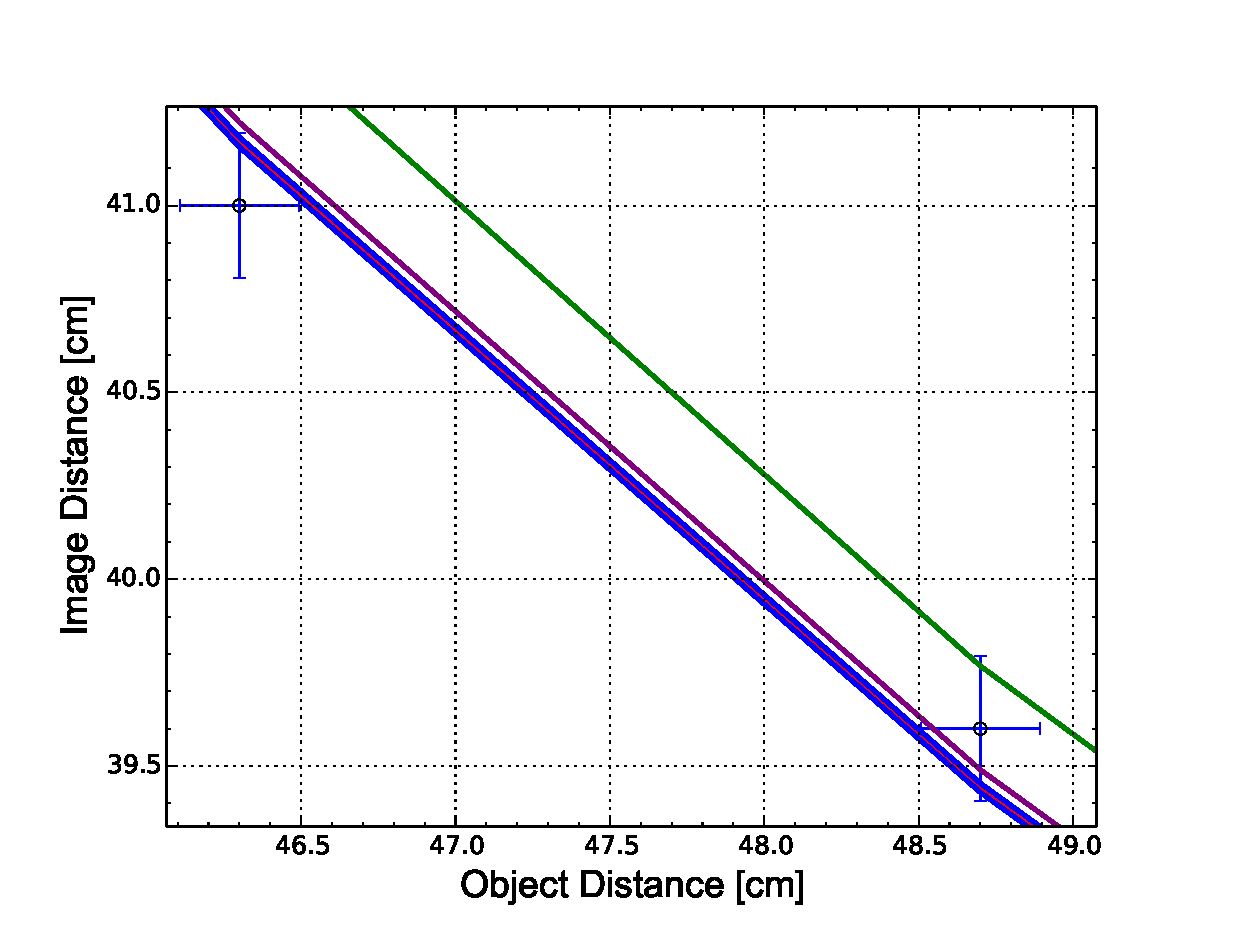
\includegraphics[scale=0.4]{zoom.eps}}
  \caption{Data from the object X lamps along with the quartz known. Red and green lines are 4 seconds and 1 second time integration, respectively. Dashed lines are drawn between the 600\,nm and 700\,nm wavelengths.}
  \label{graphs}
\end{figure*}

\begin{figure*}[ht]
  \centering
  \subfigure{\includegraphics[scale=0.4]{figure7.png}}%\quad
%  \subfigure{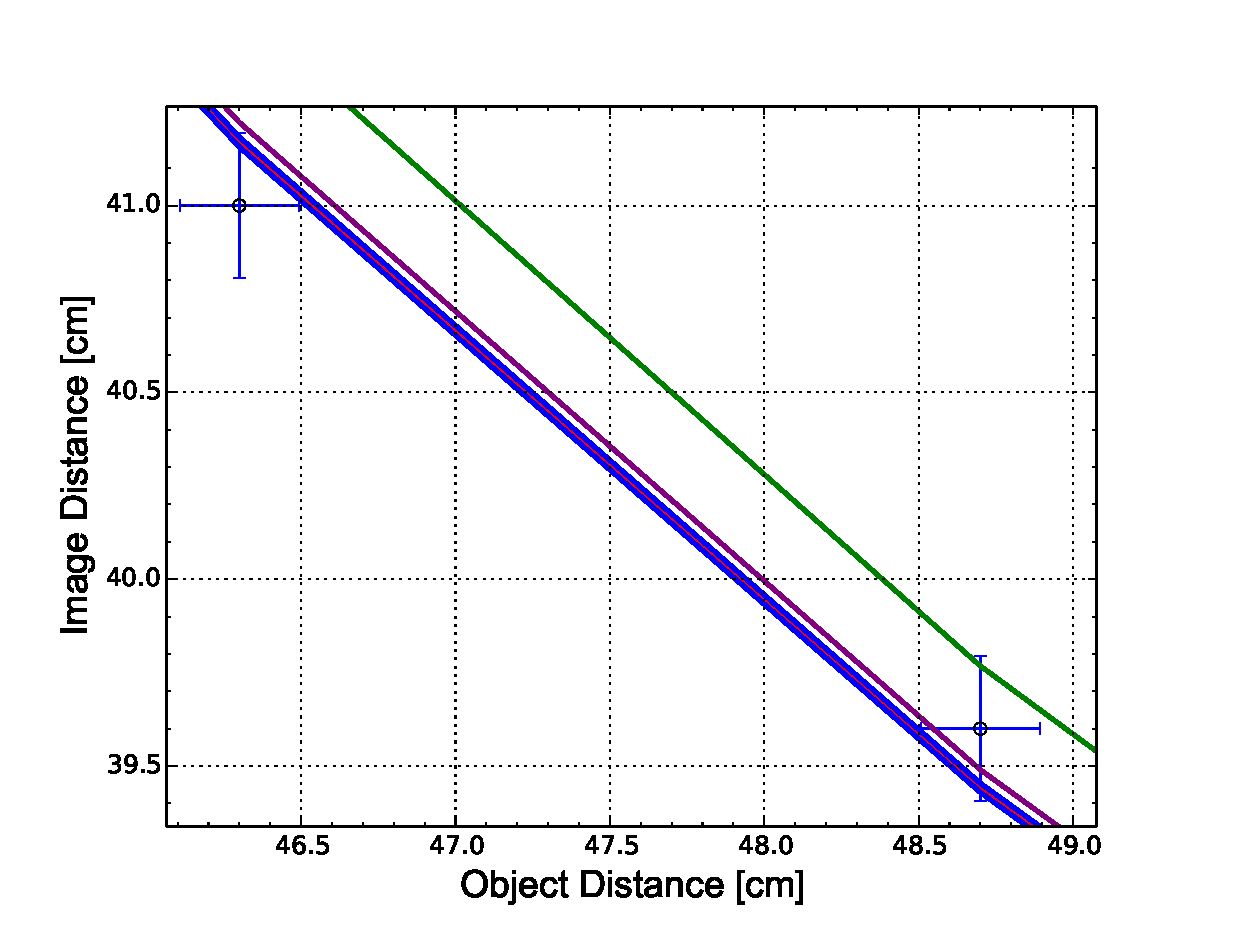
\includegraphics[scale=0.4]{zoom.eps}}
  \caption{Zoomed of above plot to show the emission line that lies within the wavelength range, optimize this plot.}
  \label{graphs}
\end{figure*}

\begin{figure*}[ht]
  \centering
  \subfigure{\includegraphics[scale=0.4]{figure_1.png}}%\quad
  \subfigure{\includegraphics[scale=0.4]{figure_4.png}}%\quad
%  \subfigure{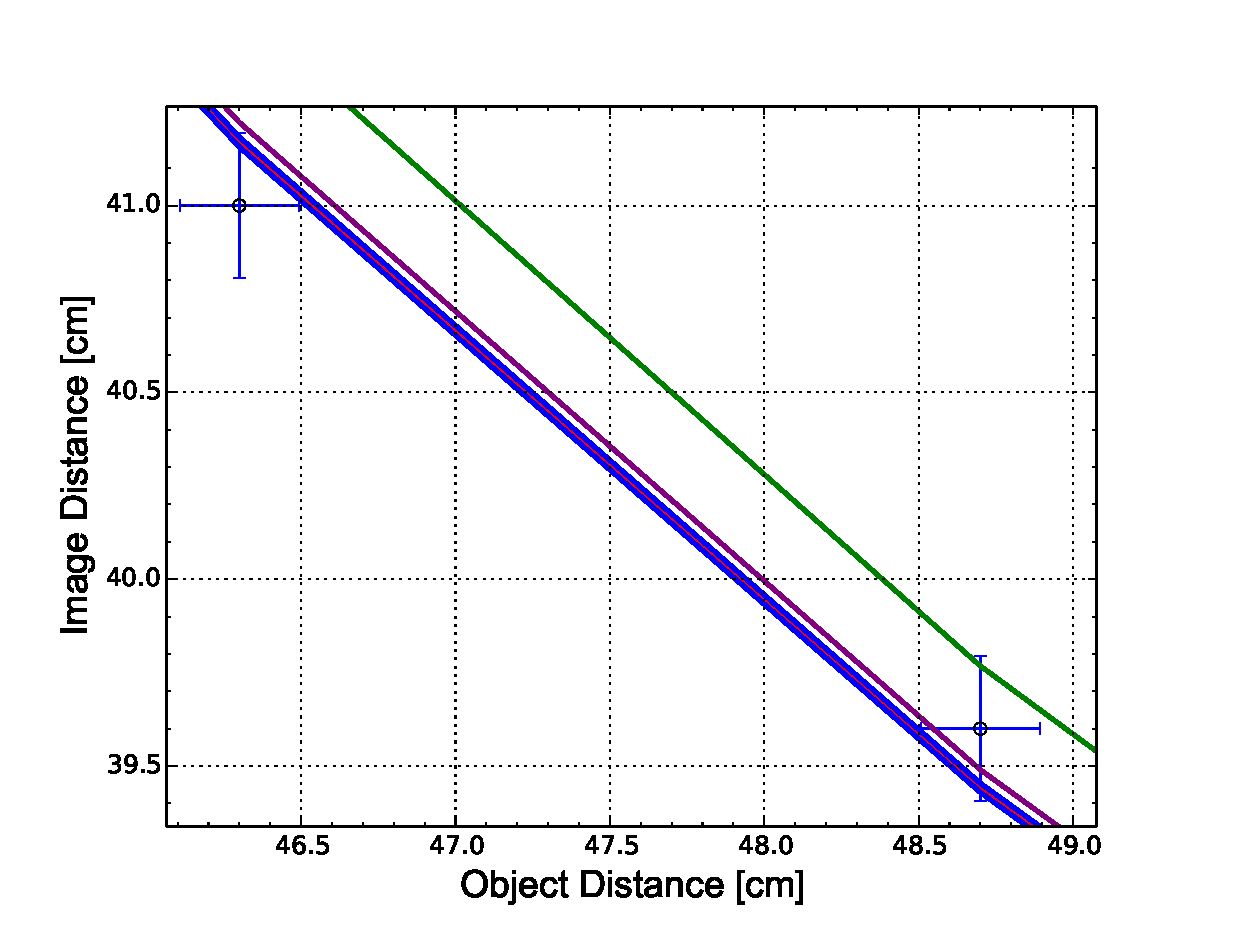
\includegraphics[scale=0.4]{zoom.eps}}
  \caption{Different spectra (left) for 5 gas lamps. Argon\,(red), helium\,(orange), hydrogen\,(yellow), mercury\,(green), neon\,(blue). Also included is the 1 second data for the object X\,(right). Fixed data (black), raw data (blue), background and dark (red).}
  \label{graphs}
\end{figure*}



\begin{itemize}
	\item{See below.}
\end{itemize}

%\acknowledgments

\section{Discussion}

The sensitivity measurements need to be redone for the respective time intervals, 1\,s and 4\,s. Although not needed, measurements for the "hotdog" lamp could be redone to include corrected time intervals.

%\vspace{5mm}

%\begin{thebibliography}{}
%
%%\bibitem[Chromey(2011)]{1}
%Chromey, Frederick R. To Measure the Sky: An Introduction to Observational Astronomy. %Cambridge: Cambridge UP, 2011. Print.
%
%\end{thebibliography}
%


%% Appendix material should be preceded with a single \appendix command.
%% There should be a \section command for each appendix. Mark appendix
%% subsections with the same markup you use in the main body of the paper.

%% Each Appendix (indicated with \section) will be lettered A, B, C, etc.
%% The equation counter will reset when it encounters the \appendix
%% command and will number appendix equations (A1), (A2), etc.


%% The reference list follows the main body and any appendices.
%% Use LaTeX's thebibliography environment to mark up your reference list.
%% Note \begin{thebibliography} is followed by an empty set of
%% curly braces.  If you forget this, LaTeX will generate the error
%% "Perhaps a missing \item?".
%%
%% thebibliography produces citations in the text using \bibitem-\cite
%% cross-referencing. Each reference is preceded by a
%% \bibitem command that defines in curly braces the KEY that corresponds
%% to the KEY in the \cite commands (see the first section above).
%% Make sure that you provide a unique KEY for every \bibitem or else the
%% paper will not LaTeX. The square brackets should contain
%% the citation text that LaTeX will insert in
%% place of the \cite commands.

%% We have used macros to produce journal name abbreviations.
%% \aastex provides a number of these for the more frequently-cited journals.
%% See the Author Guide for a list of them.

%% Note that the style of the \bibitem labels (in []) is slightly
%% different from previous examples.  The natbib system solves a host
%% of citation expression problems, but it is necessary to clearly
%% delimit the year from the author name used in the citation.
%% See the natbib documentation for more details and options.


\end{document}

%% End of file `sample.tex'.
